\section{Experiments}\label{sec:experiments}

%\aanote{this part is new.}
In this section, we empirically evaluate the proposed \textit{relational convolutional network} architecture (abbreviated RelConvNet) to assess its effectiveness at learning relational tasks. We compare this architecture to several existing relational architectures as well as general-purpose sequence models. The common input to all models is a sequence of objects $X = (x_1, \ldots, x_n) \in \reals^{n \times d}$. We evaluate against the following baselines.
\begin{itemize}
    \item \textbf{\textit{Transformer}} \citep{vaswani2017attention}. The Transformer is a powerful general-purpose sequence model. It consists of alternating self-attention and multi-layer perceptron blocks. Self-attention performs an information retrieval operation, which updates the internal representation of each object as a function of its context.
    Dot product attention is computed via $X' \gets \mathrm{Softmax}((X W_q) (X W_k)^{\intercal}) W_v X$, and the MLP is applied independently on each object's internal representation.
    The attention scores computed as an intermediate step in dot-product attention can perhaps be thought of as relations that determine what information to retrieve.
    \item \textbf{\textit{PrediNet}} \citep{shanahanExplicitlyRelationalNeural}. The PrediNet architecture is an explicitly relational architecture inspired by predicate logic. At a high-level, the PrediNet architecture computes $j$ relations between $k$ pairs of objects. The $k$ pairs of objects are selected via a learned attention operation. The ``$j$ relations'' refer to a difference between $j$-dimensional embeddings of the selected objects. More precisely, for each head $h \in [k]$, a pair of objects $E_1^h, E_2^h \in \reals^d$ is retrieved via an attention operation, and the final output of PrediNet is a set of difference relations given by $D^h = E_1^h W_s - E_2^h W_s$.
    \item \textbf{\textit{CoRelNet}} \citep{kergNeuralArchitecture2022}. The CoRelNet architecture is proposed as a minimal relational architecture distilling the core inductive biases that the authors argue are important for relational tasks. The CoRelNet module simply computes inner products between object representations and applies Softmax normalization, returning an $n \times n$ ``similarity matrix''. That is, the objects $X = (x_1, \ldots, x_n)$ are processed independently to produce embeddings $Z = (z_1, \ldots, z_n)$, and the similarity matrix is computed as $R = \mathrm{Softmax}(Z Z^\intercal)$. The similarity matrix $R$ is then flattened and passed through an MLP to produce the final output.
    \item \textbf{\textit{Graph Neural Networks}}. Graph neural networks are a class of neural network architectures which operate on graphs-structured data. A graph neural network typically receives two inputs: a graph described by a set of edges, and feature vectors for each node in the graph. GNNs can be described through the unifying framework of neural message-passing. Under this framework, graph-structured data is processed through an iterative message-passing operation given by $h_i^{(l+1)} \gets \mathrm{Update}(h_i^{(l)}, \{h_j^{(l)}\}_{j \in \calN(i)})$, where $h_i^{(0)} \gets x_i$. That is, each node's internal representation is iteratively updated as a function of its neighborhood. Here, $\mathrm{Update}$ is parameterized by a neural network, and the variation between different GNN architectures lies in the architectural design of this update process. We use Graph convolution Networks~\citep{kipfSemiSupervisedClassificationGraph2017}, Graph Attention Networks~\citep{velickovicGraphAttentionNetworks2017}, and Graph Isomorphism Networks~\citep{xuHowPowerfulAre2018} as representative GNN baselines.
\end{itemize}

%\aawarning{TODO---add RelationNet baseline?}

\subsection{Relational Games}\label{ssec:exp_relational_games}

The \textit{relational games} dataset was contributed as a benchmark for relational reasoning by~\citet{shanahanExplicitlyRelationalNeural}. It consists of a family of binary classification tasks for identifying abstract relational rules between a set of objects represented as images. The object images depict simple geometric shapes and consist of three different splits with different visual styles for evaluating out-of-distribution generalization, referred to as ``pentominoes'', ``hexominoes'', and ``stripes''. The input is a sequence of objects arranged in a $3 \times 3$ grid. Each task corresponds to some relationship between the objects, and the target is to classify whether the relationship holds among the objects in the input or not (see~\Cref{fig:relational_games_dataset}).

In our experiments, we evaluate out-of-distribution generalization by training on the pentominoes objects and evaluating on the hexominoes and stripes objects. The input to the models is presented as a sequence of $9$ objects, with each object represented as a $12 \times 12 \times 3$ RGB image. All models share the common architecture $(x_1, \ldots, x_n) \to \texttt{CNN} \to \{ \cdot \} \to \texttt{MLP} \to \hat{y}$, where $\{\cdot\}$ indicates the central module being tested. In all models, the objects are first processed independently by a CNN with a shared architecture. The processed objects are then passed to the central module of the model. The final prediction is produced by an MLP with a shared architecture. 
In this section, we focus our comparison on four models: RelConvNet (ours), CoRelNet~\citep{kergNeuralArchitecture2022}, PrediNet~\citep{shanahanExplicitlyRelationalNeural}, and a Transformer~\citep{vaswani2017attention}\footnote{The GNN baselines failed to learn the relational games tasks in a way that generalizes, often severely overfitting. For clarity of presentation, we defer results on the GNN baselines to \Cref{sec:experiments_supplement}. }.
The pentominoes split is used for training,
% We hold out 1000 samples for validation (during training) and 5000 samples for testing (after training), and use the rest as the training set. \awni{we don't show val or test accs on the pentos objects, so not relevant.}
and the hexominoes and stripes splits are used to test out-of-distribution generalization after training. 
We train for 50 epochs using the categorical cross-entropy loss and the Adam optimizer with learning rate $0.001$, $\beta_1 = 0.9, \beta_2 = 0.999, \epsilon = 10^{-7}$, and batch size $512$. For each model and task, we run 5 trials with different random seeds.
\Cref{sec:experiments_supplement} describes further experimental details about the architectures and training setup.

\begin{figure}[t]
    \centering
    \begin{subfigure}[t]{0.37\textwidth}
        \centering
        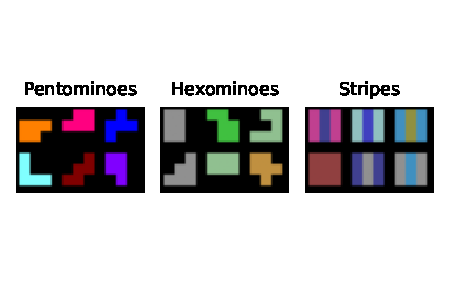
\includegraphics[width=0.99\textwidth]{figs/relational_games_objects.pdf}
        % \caption{Examples of objects from each split.}\label{fig:relational_games_objects}
    \end{subfigure}
    \begin{subfigure}[t]{0.62\textwidth}
        \centering
        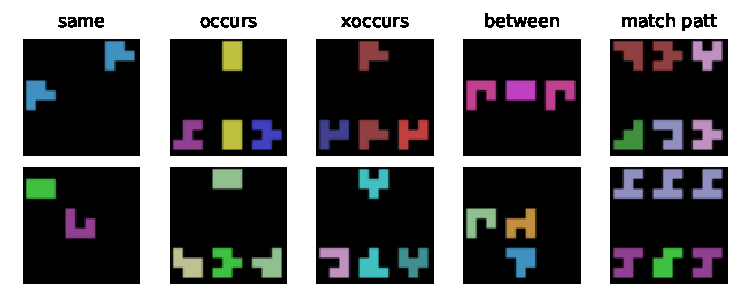
\includegraphics[width=0.95\textwidth]{figs/relational_games_tasks.pdf}
        % \caption{Examples of problem instances for each task. The top row is an example where the relation holds and the bottom row is an example where the relation does not hold.}\label{fig:relational_games_tasks}
    \end{subfigure}
    % \vskip-10pt
    \caption{Relational games dataset.~\textbf{Left} Examples of objects from each split.~\textbf{Right} Examples of problem instances for each task. The first row is an example where the relation holds and the second row is an example where the relation does not hold.}\label{fig:relational_games_dataset}
    % \vskip-12pt
\end{figure}

\textbf{Out-of-distribution generalization.}~\Cref{fig:ood_generalization} reports model performance on the two hold-out object sets after training. On the hexominoes objects, which are similar-looking to the pentominoes objects used for training, RelConvNet and CoRelNet do nearly perfectly. PrediNet and the Transformer do well on the simpler tasks, but struggle with the more difficult `match pattern' task. The `stripes' objects are visually more distinct from the objects in the training split, making generalization more difficult. We observe an overall drop in performance for all models. The drop is particularly dramatic for CoRelNet\footnote{The experiments in \citet{kergNeuralArchitecture2022} on the relational games benchmark use a technique called ``context normalization''~\citep{webbLearningRepresentationsThat2020} as a preprocessing step. We choose not to use this technique since it is an added confounder. We discuss this choice in~\Cref{sec:appendix_tcn_discussion}.}.
% We conjecture that this is due to CoRelNet's inability to model multi-dimensional relations, necessitating that all relational information is squeezed into a scalar quantity. % Or perhaps it's because of the softmax normalization?
The separation between RelConvNet and the other models is largest on the `match pattern' task of the stripes split (the most difficult task and the most difficult generalization split). Here, RelConvNet maintains a mean accuracy of 87\% while the other models drop below 65\%. We attribute this to RelConvNet's ability to naturally represent higher-order relations and model groupings of objects. The CNN baseline learns the easier `same', `between', and `occurs' tasks nearly perfectly, but completely fails to learn the more difficult `xoccurs' and `match pattern' tasks. This hard boundary suggests that explicit relational architectural inductive biases are necessary for learning more difficult relational tasks.

\begin{figure}[t]
    \centering
    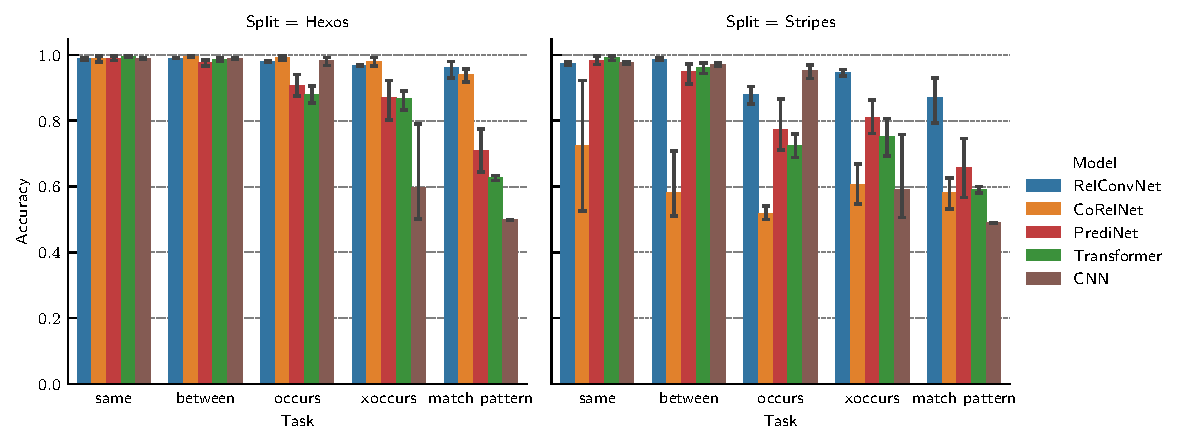
\includegraphics[width=0.95\textwidth]{figs/experiments/relgames_ood_acc.pdf}
    % \vskip-12pt
    \caption{Out-of-distribution generalization on hold-out object sets. Bar heights indicate the mean over 5 trials and the error bars indicate a bootstrap 95\% confidence interval.}\label{fig:ood_generalization}
    % \vskip-12.5pt
\end{figure}
\begin{figure}[t]
    \centering
    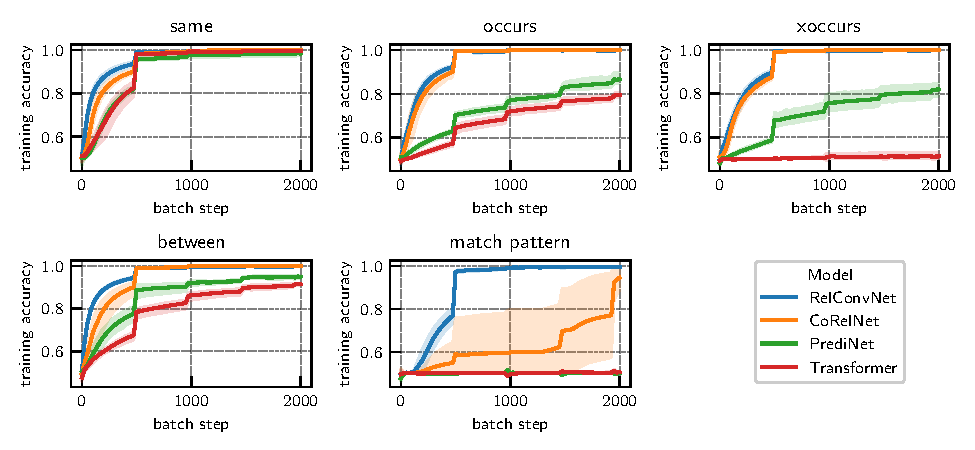
\includegraphics[width=0.95\textwidth]{figs/experiments/all_training_curves.pdf}
    % \vskip-10pt
    \caption{Training curves, up to 2,000 batch steps, for each relational games task. Solid lines indicate the mean over 5 trials and the shaded regions indicate a bootstrap 95\% confidence interval. Note that this is in-distribution (i.e., on the ``pentominoes'' split).}\label{fig:training_curves}
    % \vskip-5pt
\end{figure}

\textbf{Data efficiency.} We observe that the relational inductive biases of RelConvNet, and relational models more generally, grant a significant advantage in sample-efficiency.~\Cref{fig:training_curves} shows the training accuracy over the first 2,000 batches for each model. RelConvNet, CoRelNet, and PrediNet are explicitly relational architectures, whereas the Transformer is not. The Transformer is able to process relational information through its attention mechanism, but this information is entangled with the features of individual objects (which, for these relational tasks, is extraneous information). The Transformer consistently requires the largest amount of data to learn the relational games tasks. PrediNet tends to be more sample-efficient. RelConvNet and CoRelNet are the most sample-efficient, with RelConvNet only slightly more sample-efficient on most tasks.

On the `match pattern' task, which is the most difficult, RelConvNet is significantly more sample-efficient. We attribute this to the fact that RelConvNet is able to model higher-order relations through its relational convolution module. The `match pattern' task can be thought of as a second-order relational task---it involves computing the relational pattern in each of two groups, and comparing the two relational patterns. The relational convolution module naturally models this kind of situation since it learns representations of the relational patterns within groups of objects. %The performance we observe here indicates that the relational games dataset is in some sense saturated by models like RelConvNet and CoRelNet and that more complex relational benchmarks are needed to evaluate the limits of these models.


% \begin{table}
%     \centering
%     \caption{Performance of RelConvNet with group attention on each task.}\label{tab:relgames_groupattn_resuls}
%     \begin{tabular}{lc}
%         \toprule
%         Task & Accuracy \\
%         \midrule
%         same & $0.981 \pm 0.002$\\
%         occurs & $0.949 \pm 0.014$ \\
%         xoccurs & $0.988 \pm 0.004$\\
%         between & $1.000 \pm 0.000$ \\
%         match pattern & $0.987 \pm 0.002$\\
%         \bottomrule
%     \end{tabular}
%     \vskip-10pt
% \end{table}

% \begin{figure}
%     \centering
%         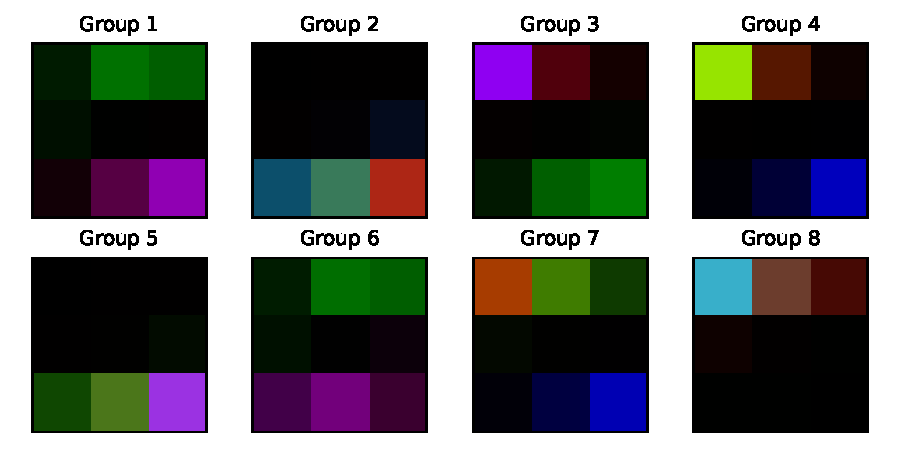
\includegraphics[width=0.65\textwidth]{figs/group_attn_figs/match_patt_group_attn_map.pdf}
%     % \vskip-10pt
%     \caption{Learned groups in the `match pattern' tasks by a 2-layer RelConvNet with group attention.}\label{fig:matchpatt_groupattn}
%     % \vskip-15pt
% \end{figure}

\begin{wrapfigure}{R}{0.5\textwidth}
    \centering
    \vskip-12pt
    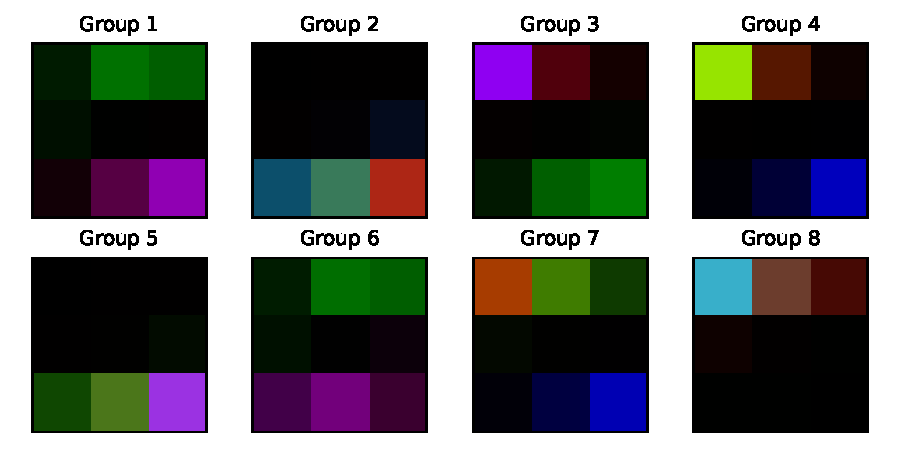
\includegraphics[width=0.5\textwidth]{figs/group_attn_figs/match_patt_group_attn_map.pdf}
    % \vskip-10pt
    \caption{Learned groups in the `match pattern' tasks by a 2-layer RelConvNet with group attention.}\label{fig:matchpatt_groupattn}
    % \vskip-15pt
\end{wrapfigure}

% \aanote{removed in-dist accuracy for relconvnet with group attn. the focus of this section is qualitative.}
\textbf{Learning groups via group attention.} Next, we analyze RelConvNet's ability to learn useful groupings through group attention in an end-to-end manner. We train a $2$-layer relational convolutional network with $8$ learned groups and a graphlet size of $3$. We group based on position by using positional embeddings for $\mathtt{key}(x_i)$.
% ~\Cref{tab:relgames_groupattn_resuls} shows the in-distribution generalization accuracy achieved by this model on each task. The model is able to learn all tasks.
In~\Cref{fig:matchpatt_groupattn}, we visualize the group attention scores $\alpha_{ij}^g$ (see~\cref{eq:group_attn}) learned from one of the training runs. For each group $g \in [n_g]$, the figure depicts a $3 \times 3$ grid representing the objects attended to in that group. Since each group contains $3$ objects, we represent the value $(\alpha_{ij}^g)_{i \in [3]}$ in the $3$-channel HSV color representation. We observe that 1) group attention learns to ignore the middle row, which contains no relevant information; and 2) the selection of objects in the top row and the bottom row is structured. In particular, group $2$ considers the relational pattern within the bottom row and group $8$ considers the relational pattern in the top row, which is exactly how a human would tackle this problem. We refer to~\Cref{fig:groupattn_entropy_reg} for an exploration of the effect of entropy regularization on group attention. We find that entropy regularization is necessary for the model to learn and causes the group attention scores to converge to interpretable discrete assignments.


\subsection{\textit{SET}: grouping and compositionality in relational reasoning}\label{ssec:experiments_set}

\textit{SET} is a card game which forms a simple but challenging relational task. The `objects' are a set of cards with four attributes, each of which can take one of three possible values. `Color' can be red, green, or purple; `number' can be one, two, or three; `shape' can be diamond, squiggle, or oval; and `fill' can be solid, striped, or empty. A `set' is a triplet of cards such that each attribute is either a) the same on all three cards, or b) different on all three cards (see~\Cref{fig:contains_set_example}).

\begin{figure}[ht]
    \centering
    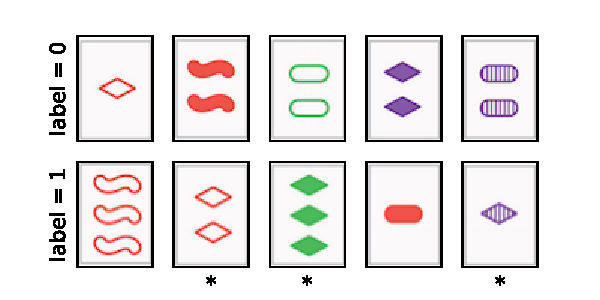
\includegraphics[width=0.4\textwidth]{figs/contains_set_example.pdf}
    \vskip-12pt
    \caption{Example of the ``contains set'' task.}\label{fig:contains_set_example}
    \vskip-7pt
\end{figure}

In \textit{SET}, the task is: given a hand of $n > 3$ cards, find a `set' among them. 
% (typically, SET is played with $k=12$, with two players competing to find a `set' first). 
This task is deceptively challenging, and is representative of the type of relational reasoning that humans excel at but machine learning systems still struggle with. To solve the task, one must process the sensory information of individual cards to identify the values of each attribute, then reason about the relational pattern in each triplet of cards.
% Importantly, this type of relational reasoning requires attending over several attributes and relations simultaneously while representing some notion of `groups'.  
The construct of relational convolutions proposed in this paper is a step towards developing machine learning systems which can perform this kind of relational reasoning.

\begin{figure}[ht]
    \centering
    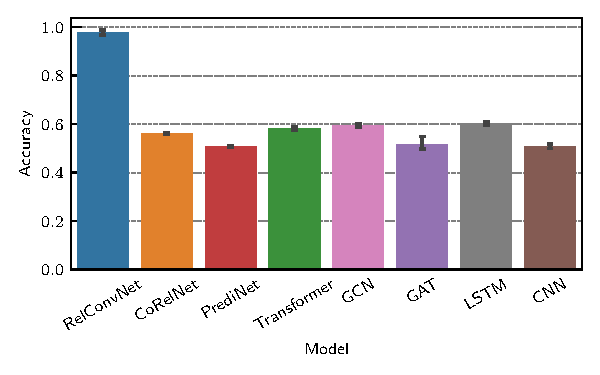
\includegraphics[width=0.4\textwidth]{figs/experiments/contains_set_acc.pdf}
    \vskip-12pt
    \caption{Hold-out test accuracy. Bar height indicates mean over 10 trials and error bars indicate 95\% confidence intervals.}\label{fig:contains_set_acc}
    \vskip-5pt
\end{figure}

In this section, we evaluate RelConvNet on a task based on \textit{SET} and compare it to several baselines. The task is: given a collection of $n=5$ images of SET cards, determine whether or not they contain a `set'. All models share the common architecture $(x_1, \ldots, x_n) \to \texttt{CNN} \to \{ \cdot \} \to \texttt{MLP} \to \hat{y}$, where $\{\cdot\}$ indicates the central module being tested. In addition to CoRelNet, PrediNet, and Transformers, we also compare RelConvNet to several GNN baselines. The CNN embedder is pre-trained on the task of classifying the four attributes of the cards and an intermediate layer is used to generate embeddings. The outupt MLP architecture is shared across all models.
%  of dimension $64$ for each card. The output MLP architecture is shared across all models, and consists of two hidden layers with $64$ and $32$ neurons, respectively, and ReLU activations. 
Further architectural details can be found in~\Cref{sec:experiments_supplement}. 

\begin{figure*}[!ht]
    \centering
    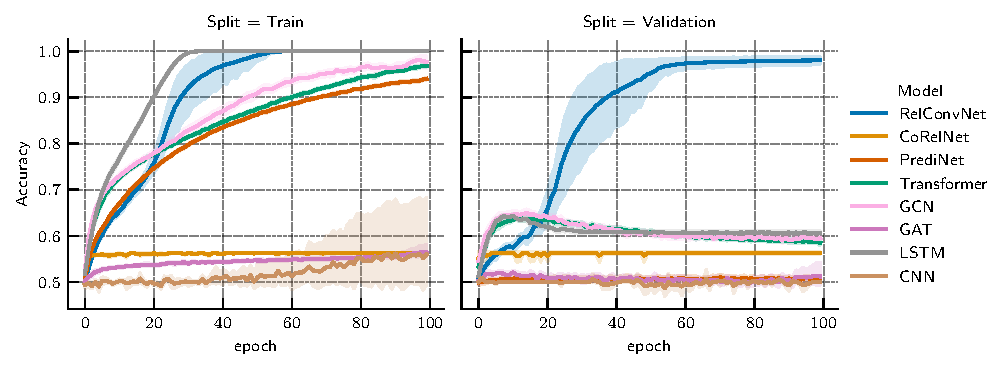
\includegraphics[width=0.8\textwidth]{figs/experiments/contains_set_training_curves.pdf}
    \vskip-10pt
    \caption{Training accuracy and validation accuracy over the course of training. Solid lines indicate mean over 10 trials and shaded regions indicates 95\% bootstrap confidence intervals.}\label{fig:contains_set_training_curves}
    \vskip-12pt
\end{figure*}

In \textit{SET}, there exists $\binom{81}{3} = 85\,320$ triplets of cards, of which $1\,080$ are a `set'. We partition the `sets' into training (70\%), validation (15\%), and test (15\%) sets. The training, validation, and test datasets are generated by sampling $k$-tuples of cards such that with probability $1/2$ the $k$-tuple does not contain a set, and with probability $1/2$ it contains a set among the corresponding partition of sets. Partitioning the data in this way allows us to measure the models' ability to ``learn the rule'' and identify new unseen `sets'.
% We train for 100 epochs with the same loss, optimizer, and batch size as the experiments in the previous section.
\Cref{fig:contains_set_acc} shows the hold-out test accuracy for each model.~\Cref{fig:contains_set_training_curves} shows the training and validation accuracy over the course of training.

We observe a sharp separation between RelConvNet and all other baselines. While RelConvNet is able to learn the task and generalize to new `sets' with near perfect accuracy (97.9\%), no other model is able to reach generalization accuracy much better than random guessing (next best is the GCN with 59.5\%). Several models are able to fit the training data, reaching near-perfect training accuracy, but they are unable to ``learn the rule'' in a way that generalizes to the validation or test sets. This suggests that while these models are powerful function approximators, they lack the inductive biases to learn hierarchical relations.

It is perhaps surprising that models like GNNs and Transformers perform poorly on these relational tasks, given their apparent ability to process relations through neural message-passing and attention, respectively. We remark that GNNs operate in a different domain compared to relational models like RelConvNet (and PrediNet, CoRelNet, etc.). In GNNs, the relations are an input to the model, received in the form of a graph, and are used to dictate the flow of information in a neural message-passing operation. By contrast, in relational convolutional networks, the input is simply a set of objects without relations---the relations need to be \textit{inferred} as part of the feature representation process. 
% Thus, GNNs operate in domains where relational information is already present (e.g., analysis of social networks, biological networks, etc.), whereas our framework aims to solve tasks which rely on relations but those relations need to be inferred end-to-end. 
This offers a partial explanation for the inability of GNNs to learn this task---GNNs are good at processing network-style relations when they are given, but may not be able to infer and hierarchically process relations when they are not given. In the case of Transformers, relations are modeled implicitly to direct information retrieval in attention, but are not encoded explicitly in the final representations.

Models like CoRelNet and PrediNet have relational inductive biases, but lack compositionality. On the other hand, deep models like Transformers and GNNs are compositional, but lack relational inductive biases. This experiment suggests that \textit{compositionality and relational inductive biases are both necessary ingredients to efficiently learn representations of higher-order relations}. RelConvNet is a compositional architecture imbued with relational inductive biases and a demonstrated ability to tackle hierarchical relational tasks.